%! alt Triangle ABC with BC = 13, CA = 10 and AB = 5, its incircle with centre I, and the dashed triangle A'B'C' obtained by the half-turn about I. Each side of A'B'C' is parallel to a side of ABC and cuts a small corner off ABC; the shaded hexagon left over is the common region, and its area is half that of ABC.
%! after_paragraph 1
%! scale 9/20
% The shared preamble of every Cevian figure. pipeline/figures turns these colours into theme-aware paint,
% and refuses any other colour, so draw only with them:
%   figink (lines and labels), figaux (construction lines), figaccent (the object the argument turns on),
%   figtint and figaccenttint (light fills).
\documentclass[border=1.5pt]{standalone}
\usepackage{tkz-euclide}
\definecolor{figink}{RGB}{0,0,0}
\definecolor{figaux}{RGB}{85,85,85}
\definecolor{figaccent}{RGB}{192,57,43}
\definecolor{figtint}{RGB}{221,221,221}
\definecolor{figaccenttint}{RGB}{245,213,208}
% tkz-euclide's defaults draw circles, compasses and marks in 50% grey and fill points with a tint.
\makeatletter
\def\tkz@otherlinecolor{figink}
\def\tkz@euc@circlecolor{figink}
\def\tkz@euc@compasscolor{figink}
\def\tkz@euc@mkcolor{figink}
\def\tkz@mk@fill{figink}
\def\tkz@euc@pointfillcolor{figink}
\makeatother
\tkzSetUpLine[color=figink,line width=.7pt]
\tkzSetUpArc[color=figink,line width=.7pt]
\tkzSetUpCompass[color=figink,line width=.5pt]
\tkzSetUpPoint[color=figink,fill=figink,size=3.1pt]
\tikzset{
  every picture/.style={line cap=round,line join=round,color=figink},
  circle style/.append style={color=figink,line width=.7pt},
  aux/.style={color=figaux,line width=.45pt,dash pattern=on 2.6pt off 2pt},
  key/.style={color=figaccent,line width=1pt},
  mk/.style={color=figink,line width=.5pt},
  lbl/.style={color=figink,inner sep=2.2pt},
  len/.style={color=figink,inner sep=1.5pt,font=\small},
}

\begin{document}
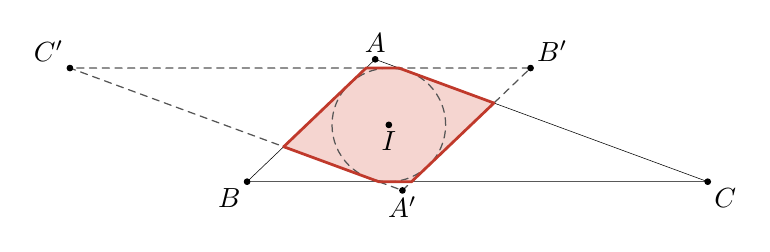
\begin{tikzpicture}
\tkzDefPoint(0.0,0.0){B} %! B = (0, 0)
\tkzDefPoint(5.8500000,0.0){C} %! C = (13, 0)
\tkzDefPoint(1.6269231,1.5542269){A} %! A = (47/13, 12*sqrt(14)/13)
\tkzDefPoint(1.8000000,0.72160535){I} %! I = incentre(A, B, C)
\tkzDefPoint(1.8000000,0.0){D} %! D = foot(I, B, C)
\tkzDefPoint(1.9730769,-0.11101621){Ap} %! Ap = lerp(A, I, 2)
\tkzDefPoint(3.6000000,1.4432107){Bp} %! Bp = lerp(B, I, 2)
\tkzDefPoint(-2.2500000,1.4432107){Cp} %! Cp = lerp(C, I, 2)
\tkzDefPoint(1.5107143,1.4432107){Ha} %! Ha = meet(Bp, Cp, A, B)
\tkzDefPoint(1.9285714,1.4432107){Hb} %! Hb = meet(Bp, Cp, A, C)
\tkzDefPoint(1.6714286,0.0){Hc} %! Hc = meet(Cp, Ap, B, C)
\tkzDefPoint(0.46483516,0.44406483){Hd} %! Hd = meet(Cp, Ap, A, B)
\tkzDefPoint(2.0892857,0.0){He} %! He = meet(Ap, Bp, B, C)
\tkzDefPoint(3.1351648,0.99914587){Hf} %! Hf = meet(Ap, Bp, C, A)
%! fact midpoint(I, A, Ap)
%! fact midpoint(I, B, Bp)
%! fact midpoint(I, C, Cp)
%! fact parallel(Bp, Cp, B, C)
%! fact parallel(Cp, Ap, C, A)
%! fact parallel(Ap, Bp, A, B)
%! fact dist(Ha, A) / dist(A, B) == 1 - dist(B, C) / ((dist(A, B) + dist(B, C) + dist(C, A)) / 2)
%! fact area(Hc, He, Hf, Hb, Ha, Hd) == area(A, B, C) / 2
%! example dist(B, C) == 13
%! example dist(C, A) == 10
%! example dist(A, B) == 5
\tkzFillPolygon[color=figaccenttint](Hc,He,Hf,Hb,Ha,Hd)
\tkzDrawCircle[aux](I,D)
\tkzDrawPolygon[aux](Ap,Bp,Cp)
\tkzDrawPolygon(A,B,C)
\tkzDrawPolygon[key](Hc,He,Hf,Hb,Ha,Hd)
\tkzDrawPoints(A,B,C,I,Ap,Bp,Cp)
\tkzLabelPoint[above,lbl](A){$A$}
\tkzLabelPoint[below left,lbl](B){$B$}
\tkzLabelPoint[below right,lbl](C){$C$}
\tkzLabelPoint[below,lbl](I){$I$}
\tkzLabelPoint[below,lbl](Ap){$A'$}
\tkzLabelPoint[above right,lbl](Bp){$B'$}
\tkzLabelPoint[above left,lbl](Cp){$C'$}
\end{tikzpicture}
\end{document}
